\chapter{Hong Kong}
\section*{30 octobre 2015}
Je tente de passer la frontière entre la Chine et HK en vélo mais c'est impossible, obligé de mettre le vélo dans un bus \newline
 Belles pistes cyclables sur quelques dizaines de km ensuite \newline
 \newline
\centerline{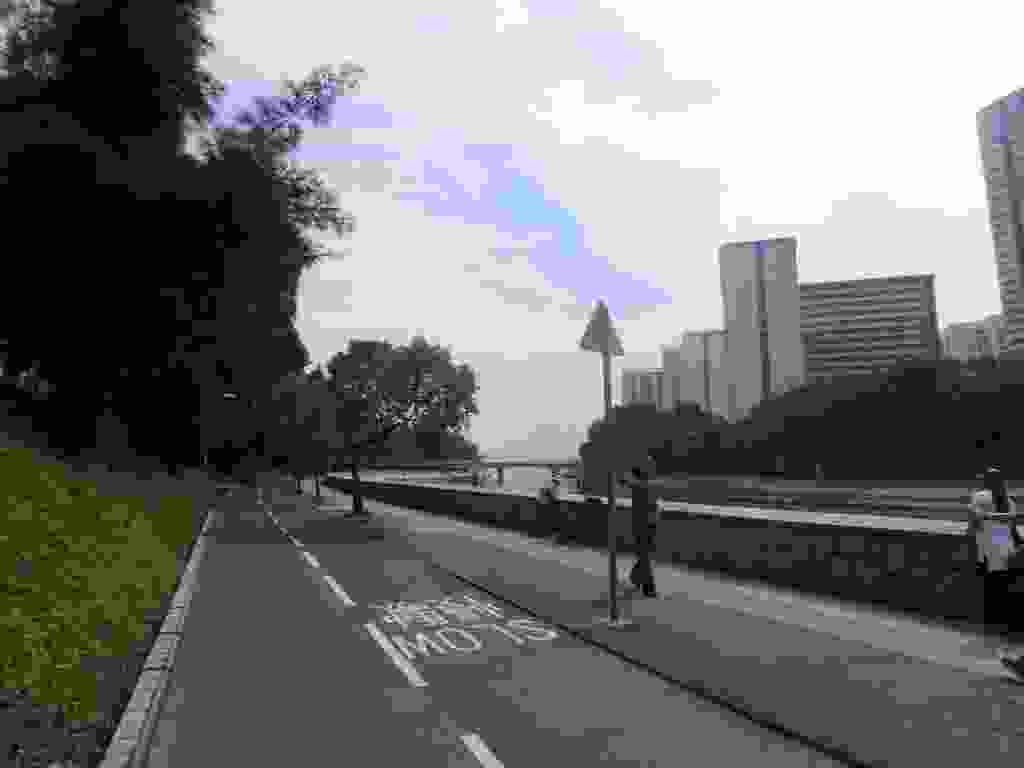
\includegraphics[width=\mywidth]{../wp-content/uploads/2015/10/wpid-oi000043-1024x768.jpg} } 
 \newline
 \newline
\centerline{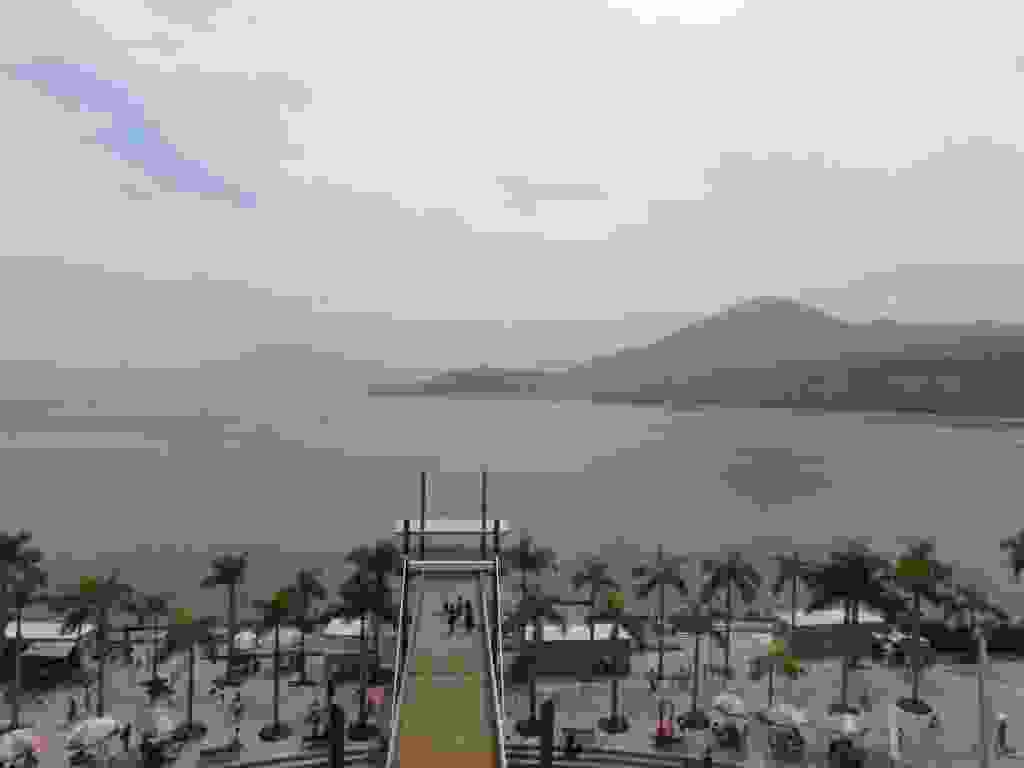
\includegraphics[width=\mywidth]{../wp-content/uploads/2015/10/wpid-oi000045-1024x768.jpg} } 
 \newline
 \newline
\centerline{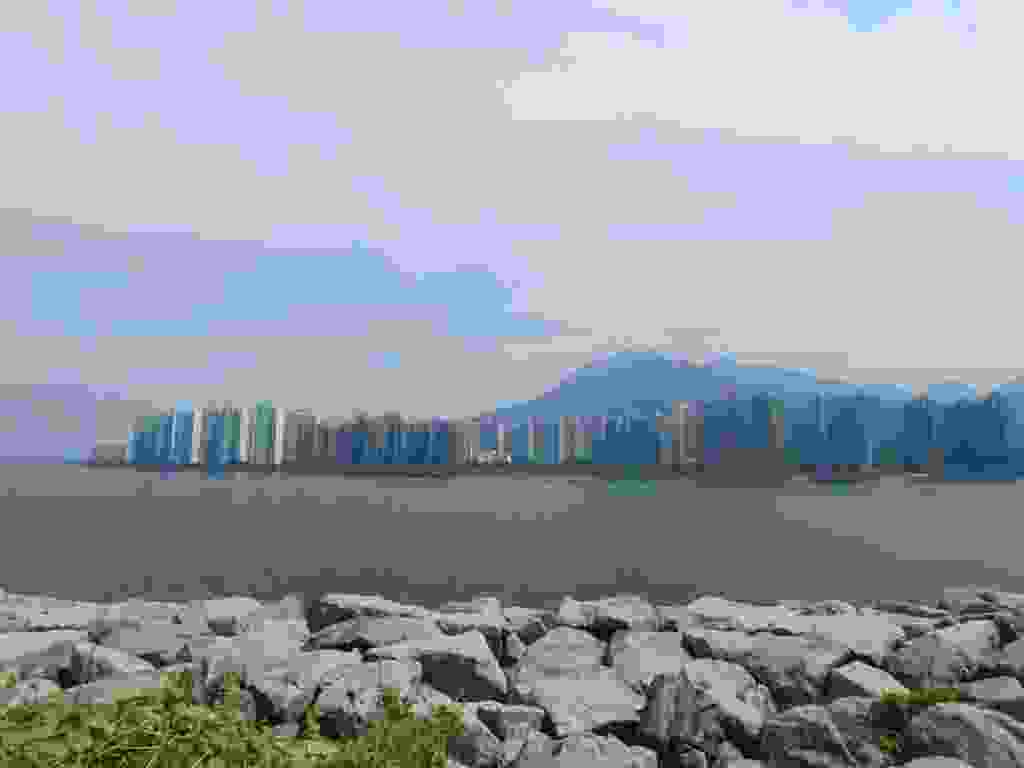
\includegraphics[width=\mywidth]{../wp-content/uploads/2015/10/wpid-oi000048-1024x768.jpg} } 
 \newline
 Premier jour dans le parc de Sai Kung à l'est des Nouveaux Territoires, partie de HK sur le continent. Forêts, petites plages et emplacements de camping gratuits, avec un climat parfait à cette saison \newline
 \newline
\centerline{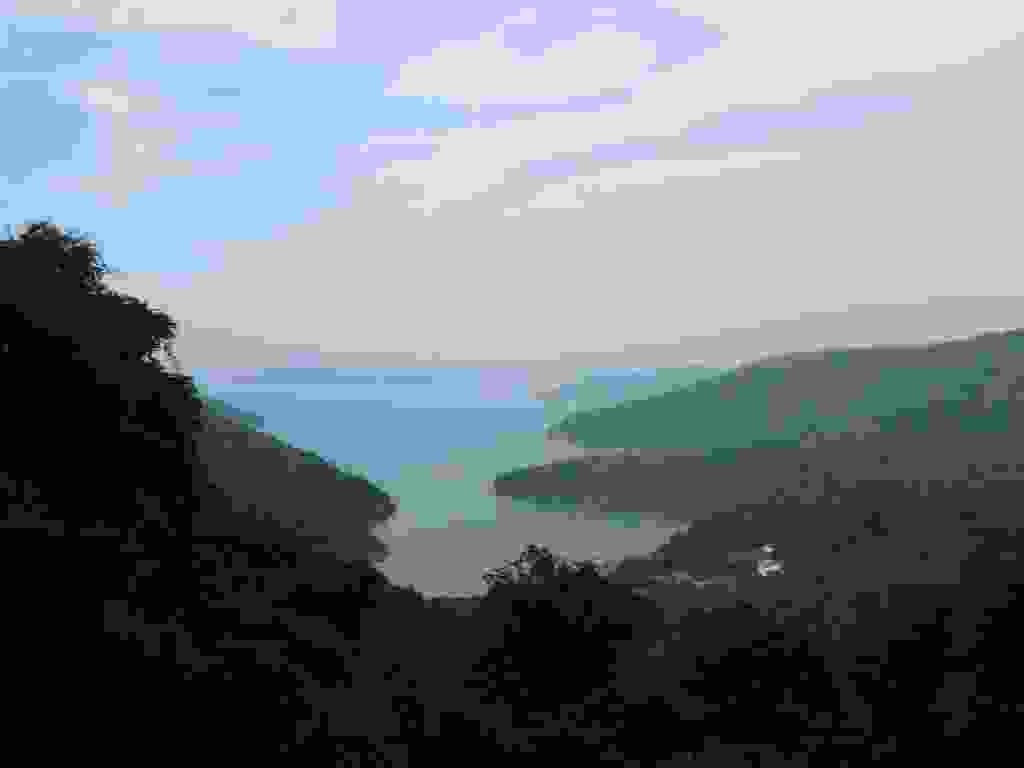
\includegraphics[width=\mywidth]{../wp-content/uploads/2015/10/wpid-oi000053-1024x768.jpg} } 
 \newline
 \newline
\centerline{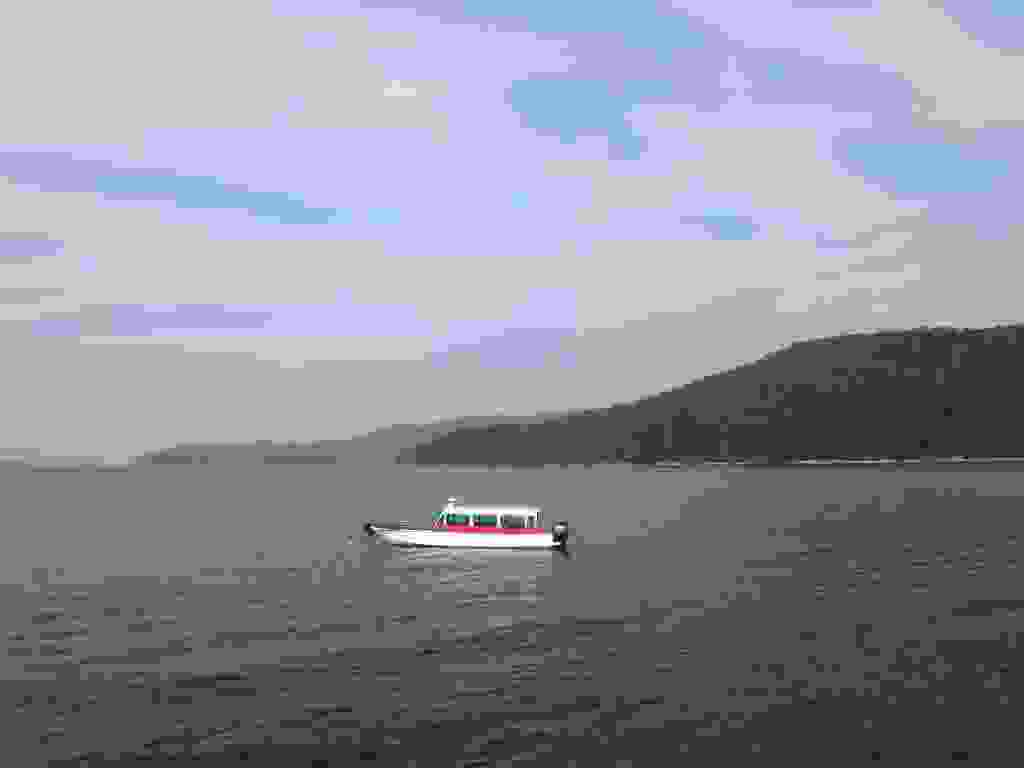
\includegraphics[width=\mywidth]{../wp-content/uploads/2015/10/wpid-oi000054-1024x768.jpg} } 
 \newline
 \newline
\centerline{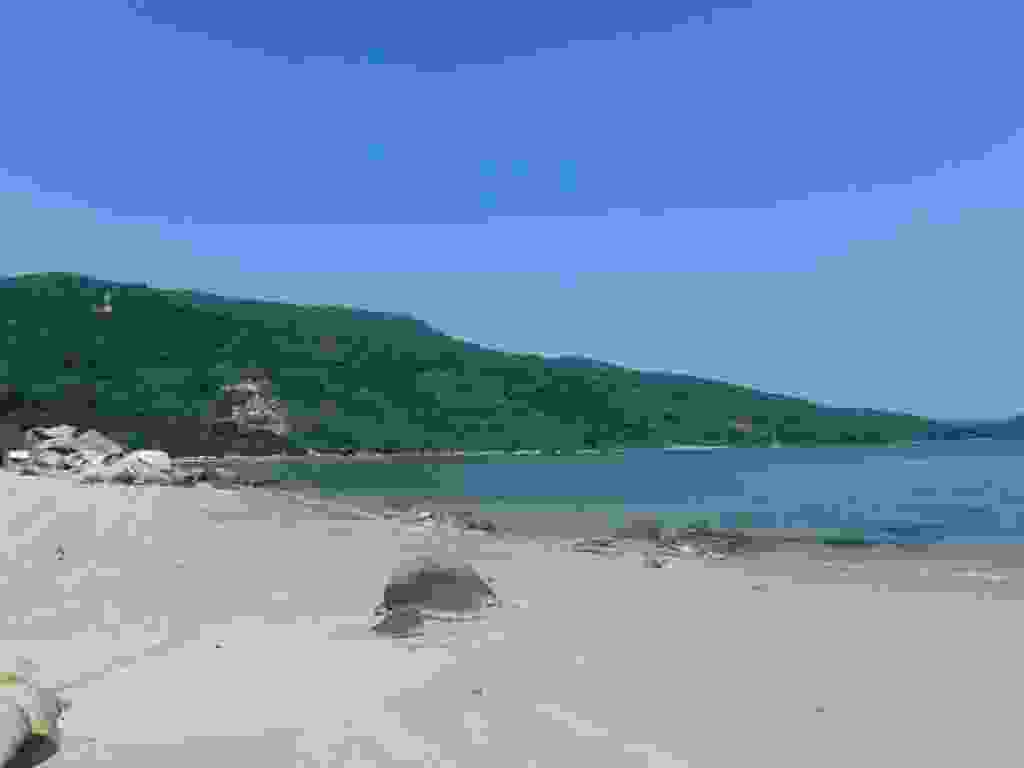
\includegraphics[width=\mywidth]{../wp-content/uploads/2015/10/wpid-oi000058-1024x768.jpg} } 
 \newline
 \newline
\centerline{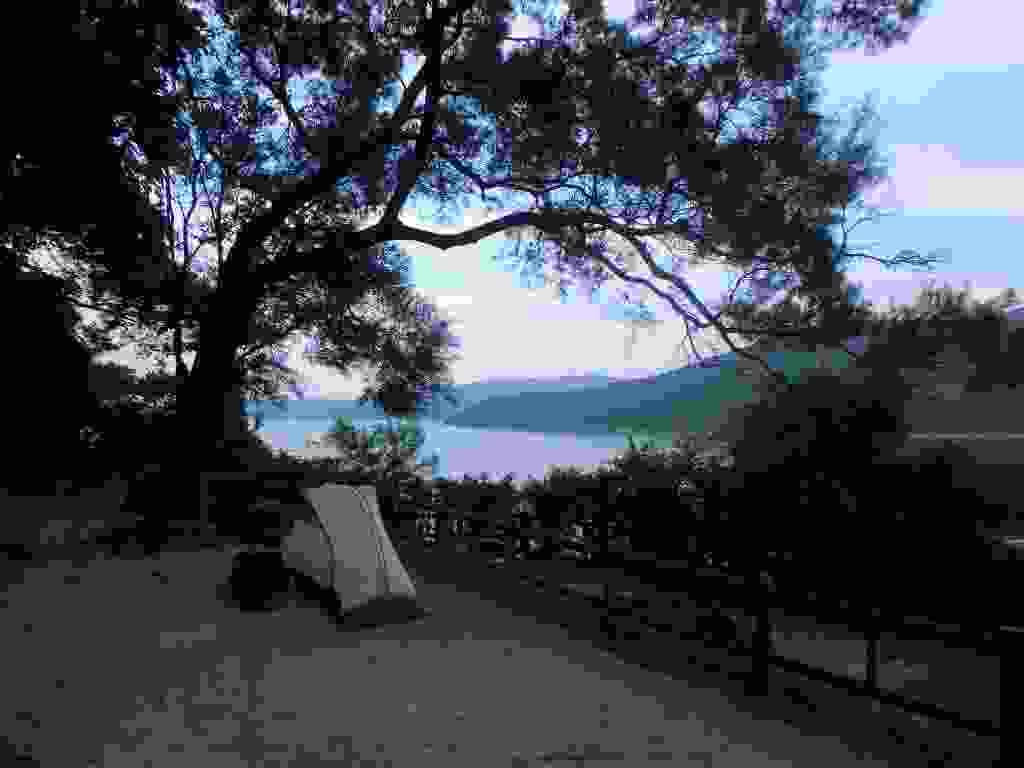
\includegraphics[width=\mywidth]{../wp-content/uploads/2015/10/wpid-oi000057-1024x768.jpg} } 
 \newline
 Port de Sai Kung \newline
 \newline
\centerline{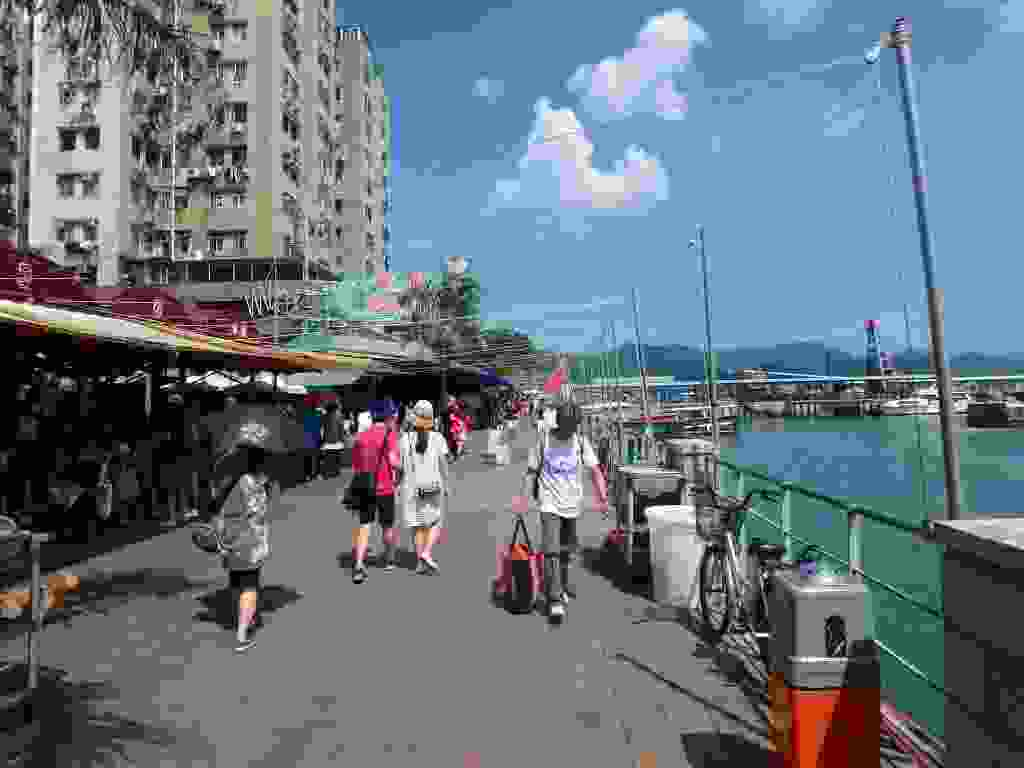
\includegraphics[width=\mywidth]{../wp-content/uploads/2015/10/wpid-oi000063-1024x768.jpg} } 
 \newline
 \newline
\centerline{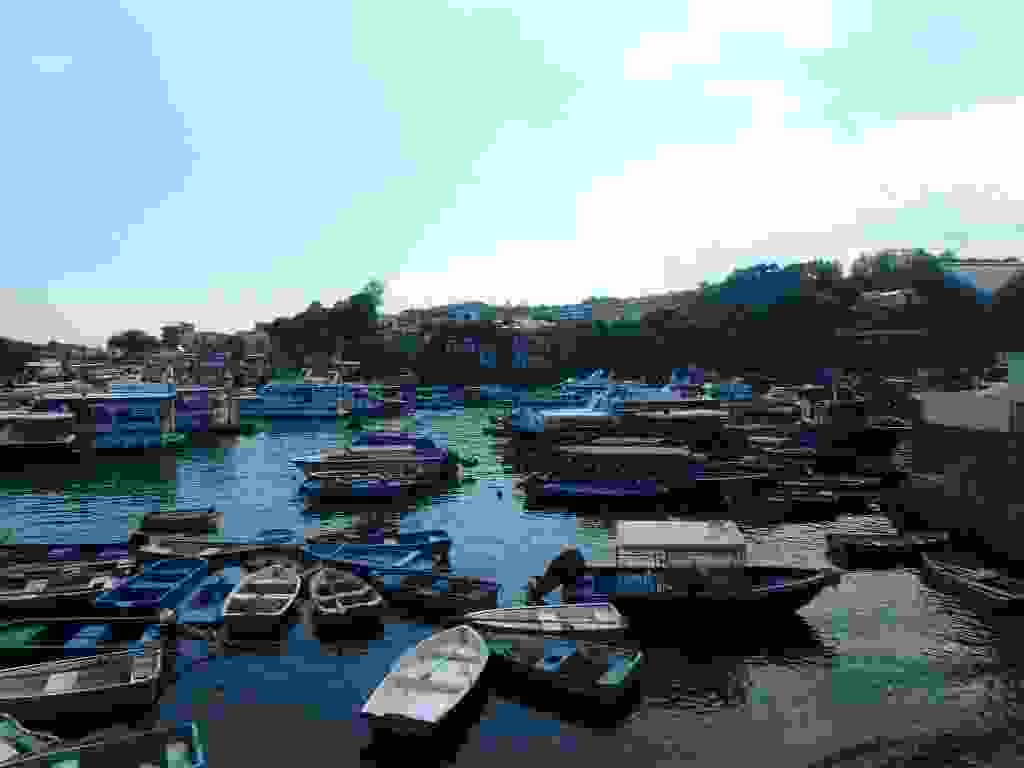
\includegraphics[width=\mywidth]{../wp-content/uploads/2015/10/wpid-oi000065-1024x768.jpg} } 
 \newline
 Je rejoins le centre, échangeurs énormes, routes surélevées dans tous les sens, certaines interdites aux vélos, le GPS est bien utile \newline
 2 jours à l'hôtel dans le quartier de Kowloon, au 11e étage d'un immeuble. Tellement exigu que le vélo doit rester dehors \newline
 \newline
\centerline{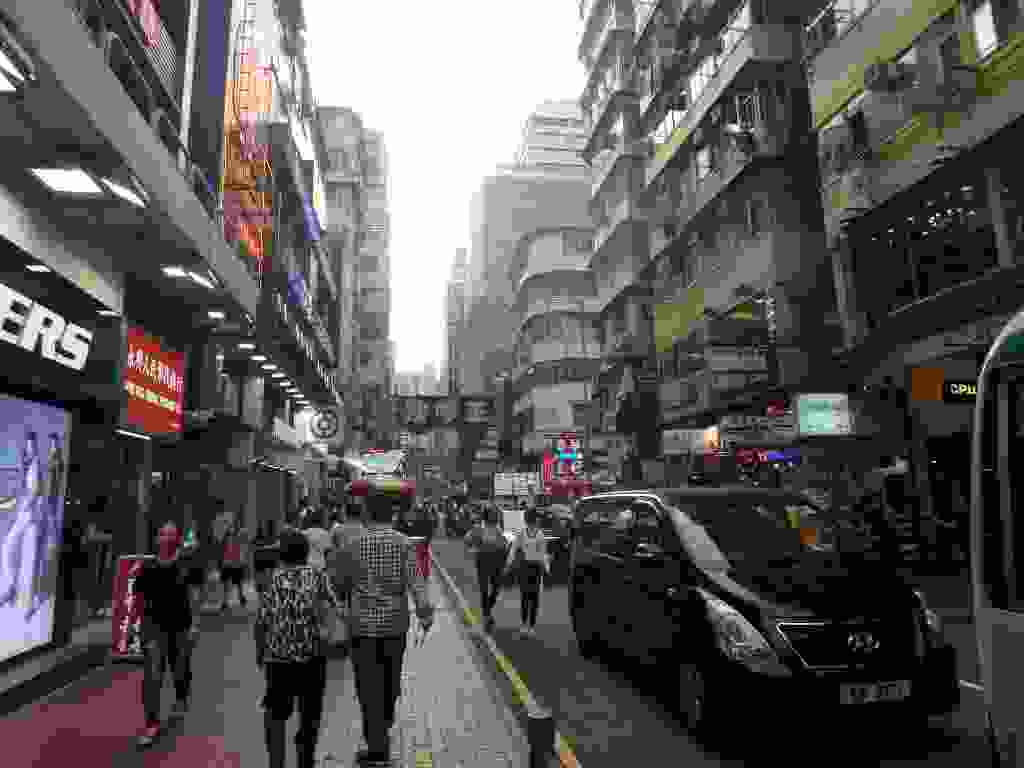
\includegraphics[width=\mywidth]{../wp-content/uploads/2015/10/wpid-oi000069-1024x768.jpg} } 
 \newline
 \newline
\centerline{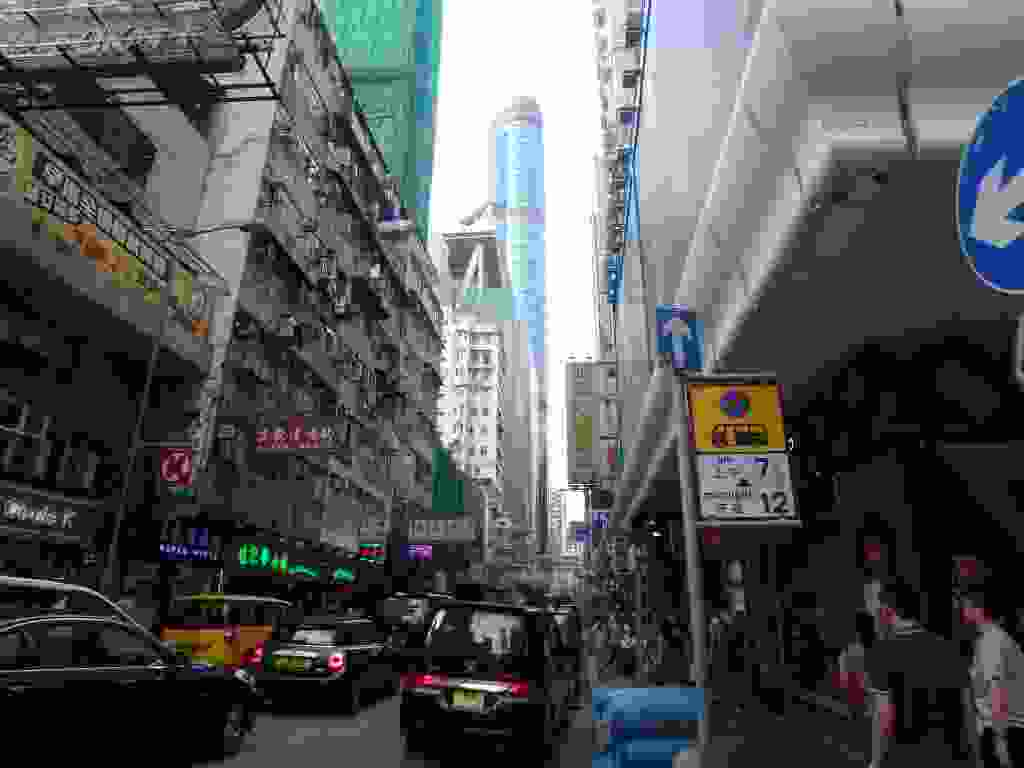
\includegraphics[width=\mywidth]{../wp-content/uploads/2015/10/wpid-oi0001201-1024x768.jpg} } 
 \newline
 \newline
\centerline{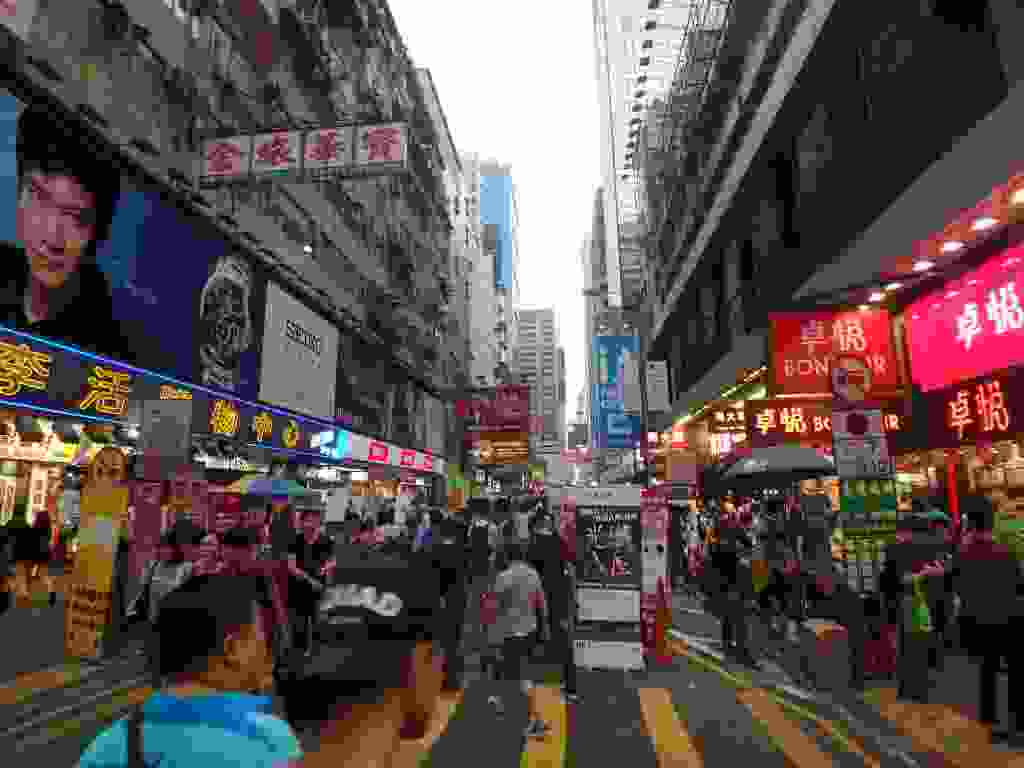
\includegraphics[width=\mywidth]{../wp-content/uploads/2015/10/wpid-oi0001221-1024x768.jpg} } 
 \newline
 Ensuite, Kévin m'héberge en couchsurfing dans l'appartement où il vit avec sa mère et son frère, superbe accueil avec un bon repas de spécialités locales \newline
 \newline
\centerline{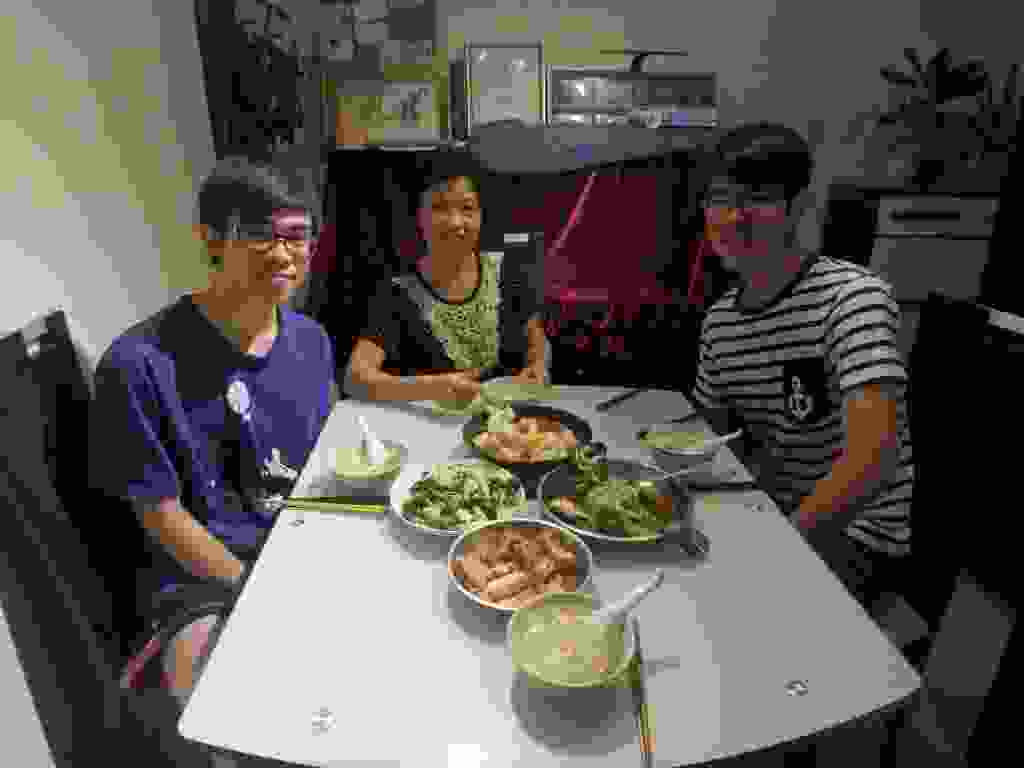
\includegraphics[width=\mywidth]{../wp-content/uploads/2015/10/wpid-oi000082-1024x768.jpg} } 
 \newline
 On va sur l'île de Hong Kong, montée à Victoria Peak \newline
 \newline
\centerline{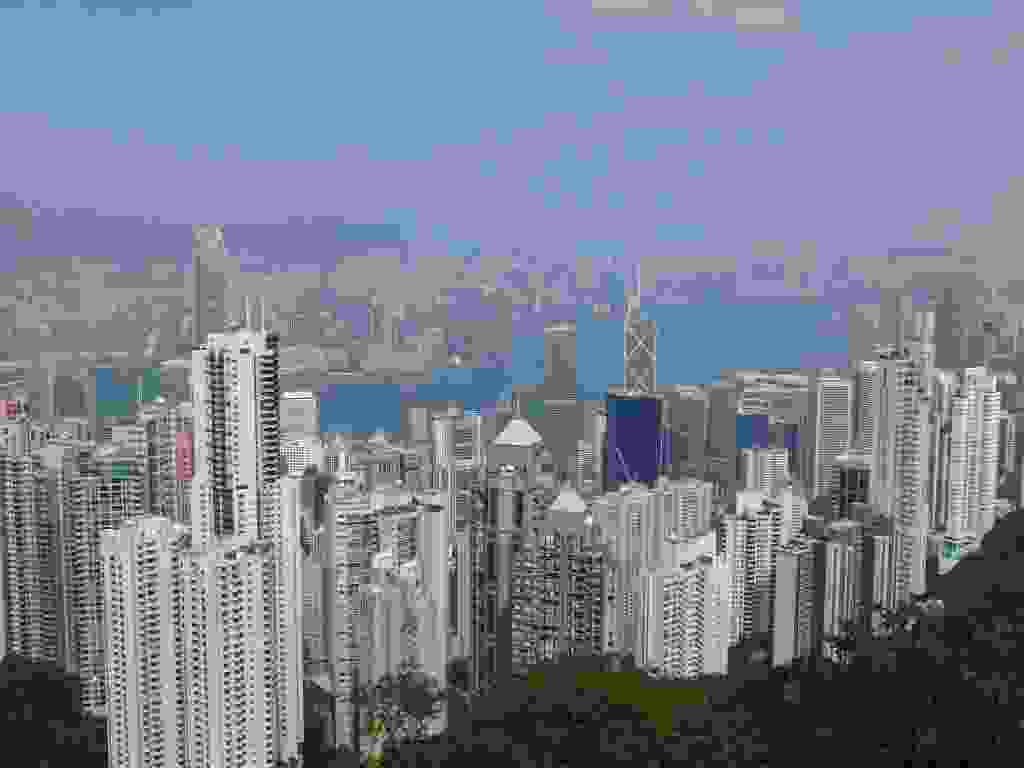
\includegraphics[width=\mywidth]{../wp-content/uploads/2015/10/wpid-oi000090-1024x768.jpg} } 
 \newline
 Balade pour voir le port d'Aberdeen au sud \newline
 \newline
\centerline{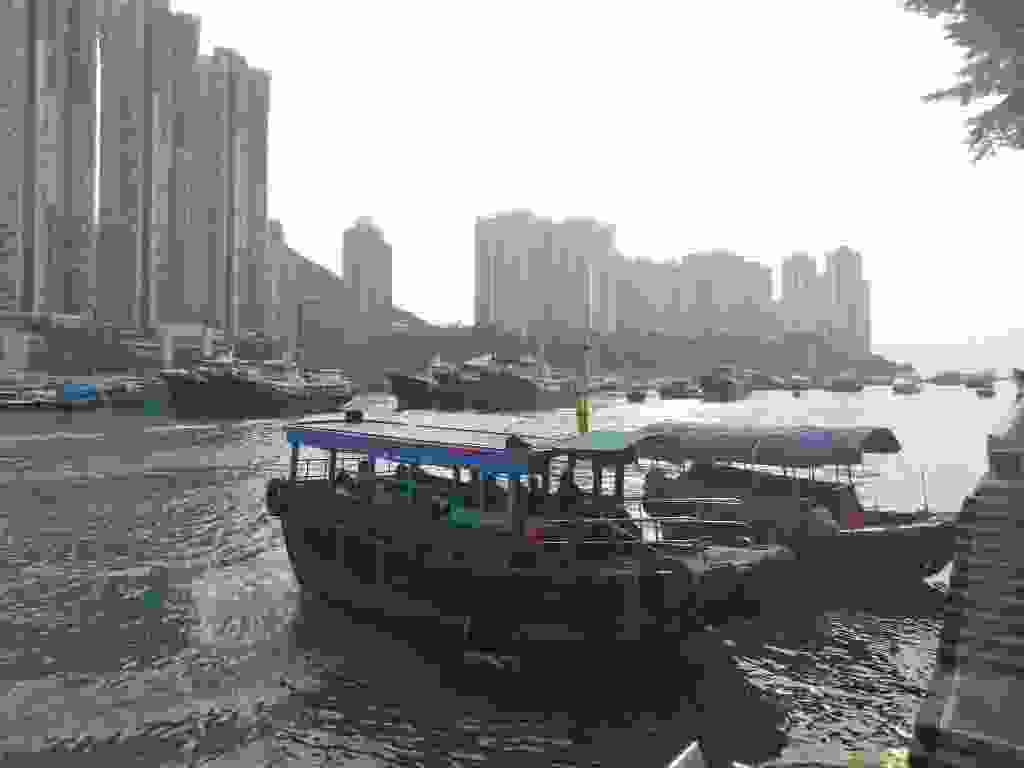
\includegraphics[width=\mywidth]{../wp-content/uploads/2015/10/wpid-oi000098-1024x768.jpg} } 
 \newline
 \newline
\centerline{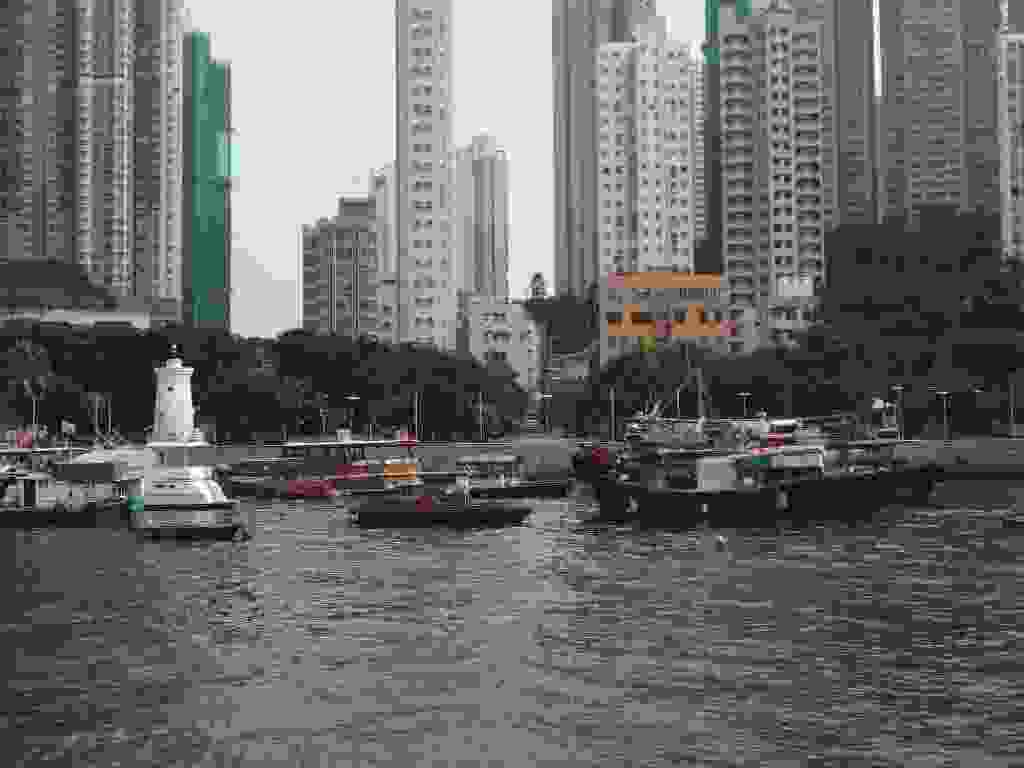
\includegraphics[width=\mywidth]{../wp-content/uploads/2015/10/wpid-oi000096-1024x768.jpg} } 
 \newline
 \newline
\centerline{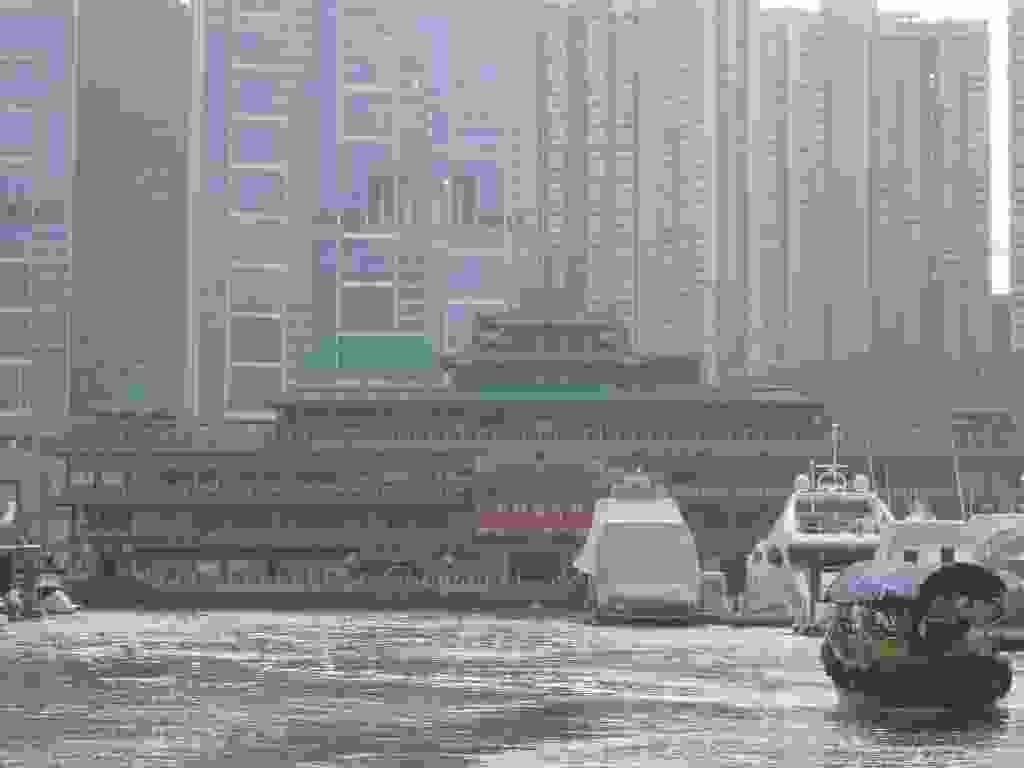
\includegraphics[width=\mywidth]{../wp-content/uploads/2015/10/wpid-oi000106-1024x768.jpg} } 
 \newline
 Petit temple, je ne sais pas si c'est bouddhiste ou taoïste \newline
 \newline
\centerline{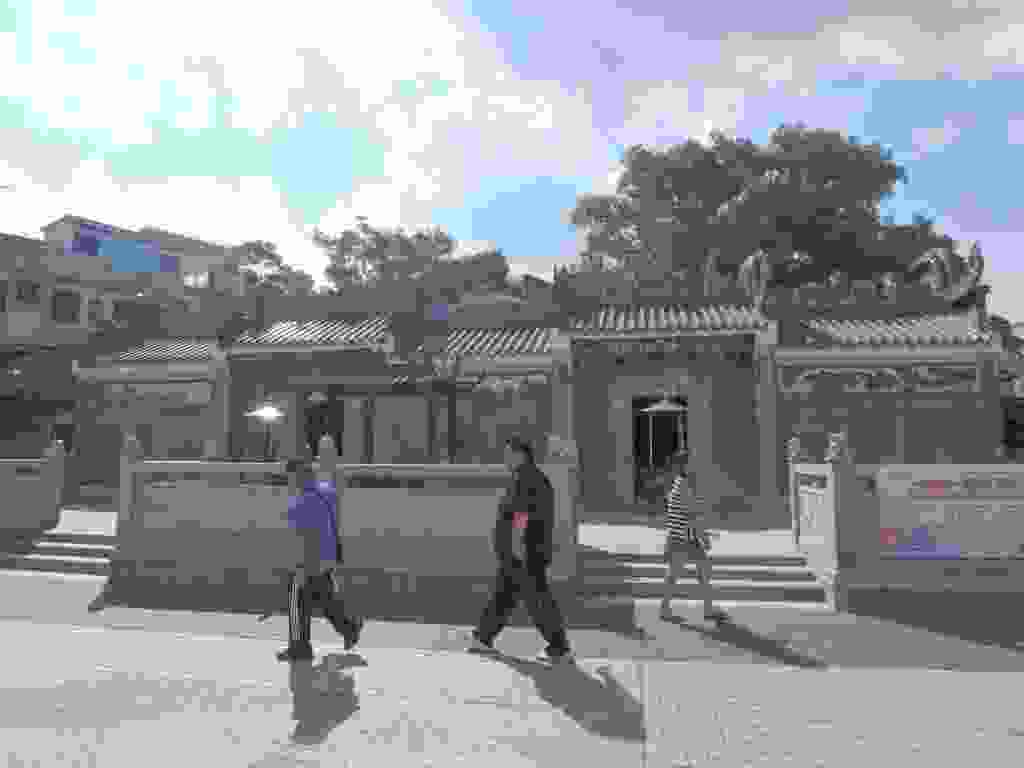
\includegraphics[width=\mywidth]{../wp-content/uploads/2015/10/wpid-oi000066-1024x768.jpg} } 
 \newline
 \newline
\centerline{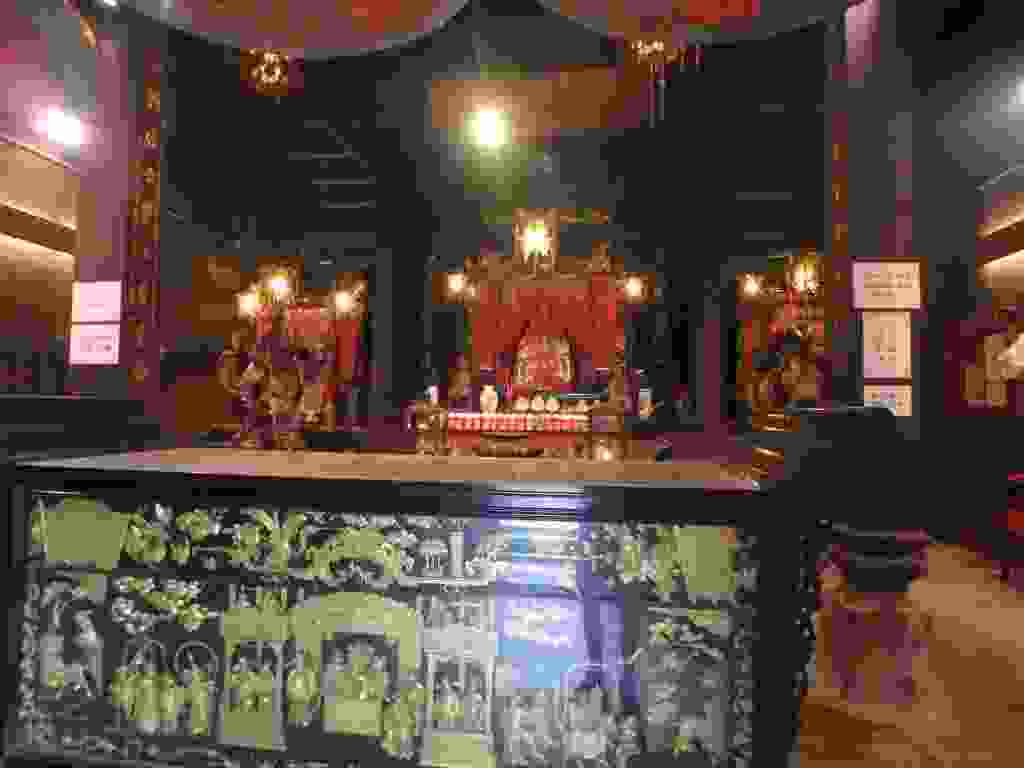
\includegraphics[width=\mywidth]{../wp-content/uploads/2015/10/wpid-oi000092-1024x768.jpg} } 
 \newline
 Le long de la rivière entre Hong Kong Island et Kowloon \newline
 \newline
\centerline{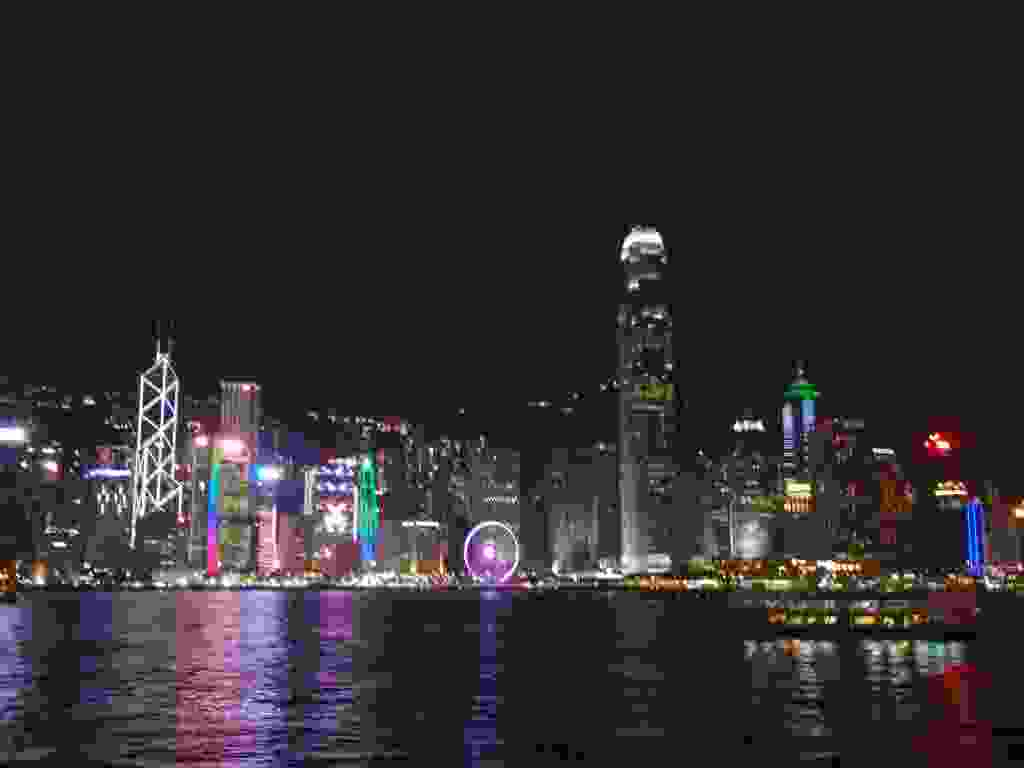
\includegraphics[width=\mywidth]{../wp-content/uploads/2015/10/wpid-oi000072-1024x768.jpg} } 
 \newline
 \newline
\centerline{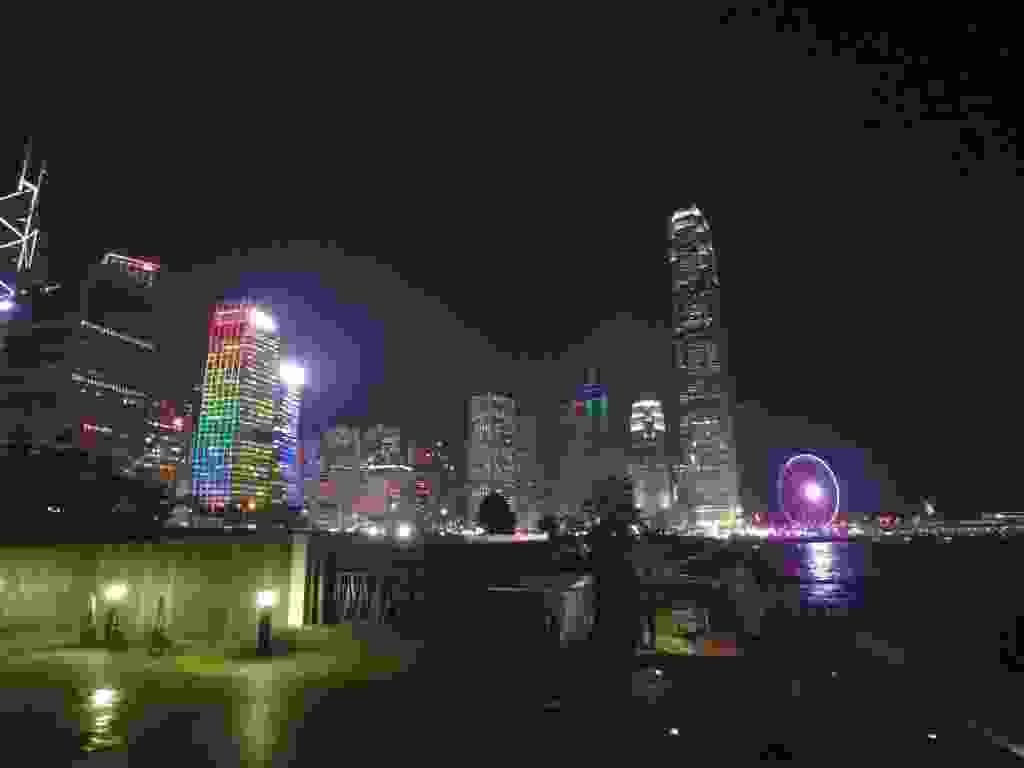
\includegraphics[width=\mywidth]{../wp-content/uploads/2015/10/wpid-oi000113-1024x768.jpg} } 
 \newline
 Traversée de Hong Kong Island d'ouest en est en tramway \newline
 \newline
\centerline{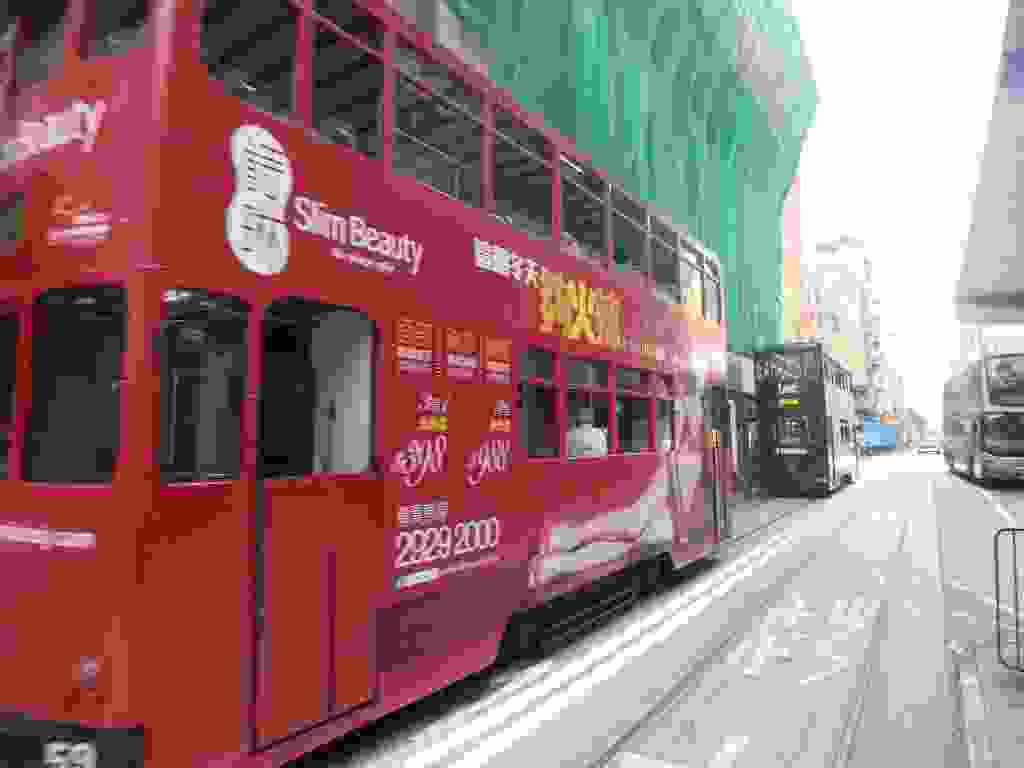
\includegraphics[width=\mywidth]{../wp-content/uploads/2015/10/wpid-oi0000741-1024x768.jpg} } 
 \newline
 \newline
\centerline{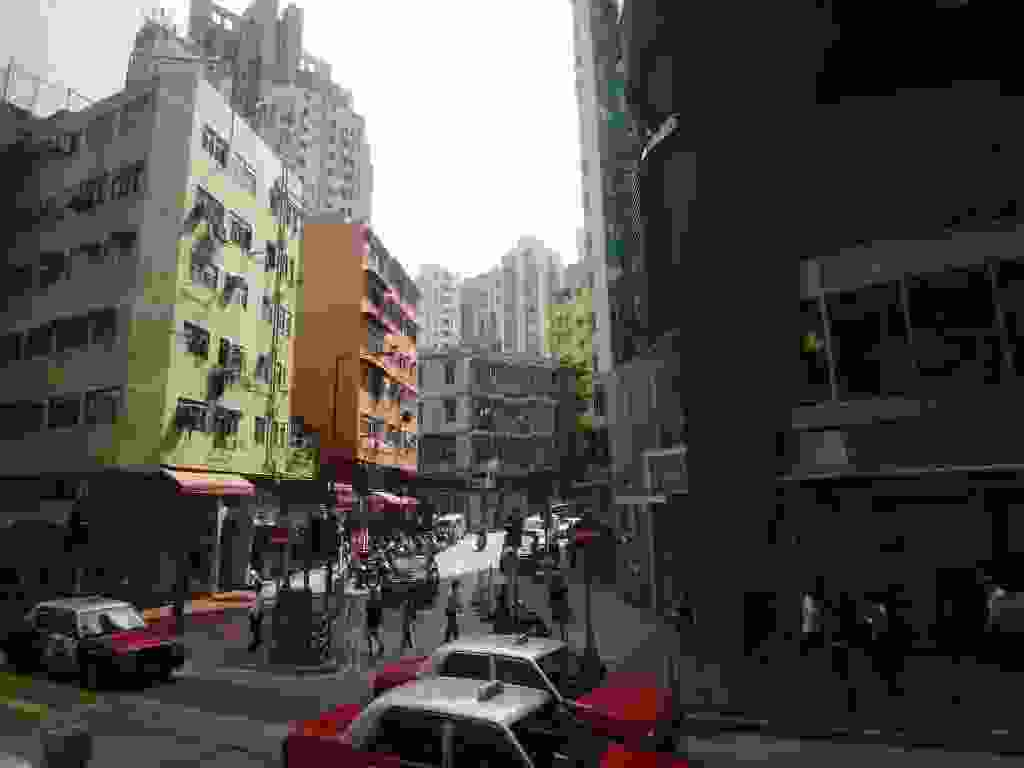
\includegraphics[width=\mywidth]{../wp-content/uploads/2015/10/wpid-oi000087-1024x768.jpg} } 
 \newline
 \newline
\centerline{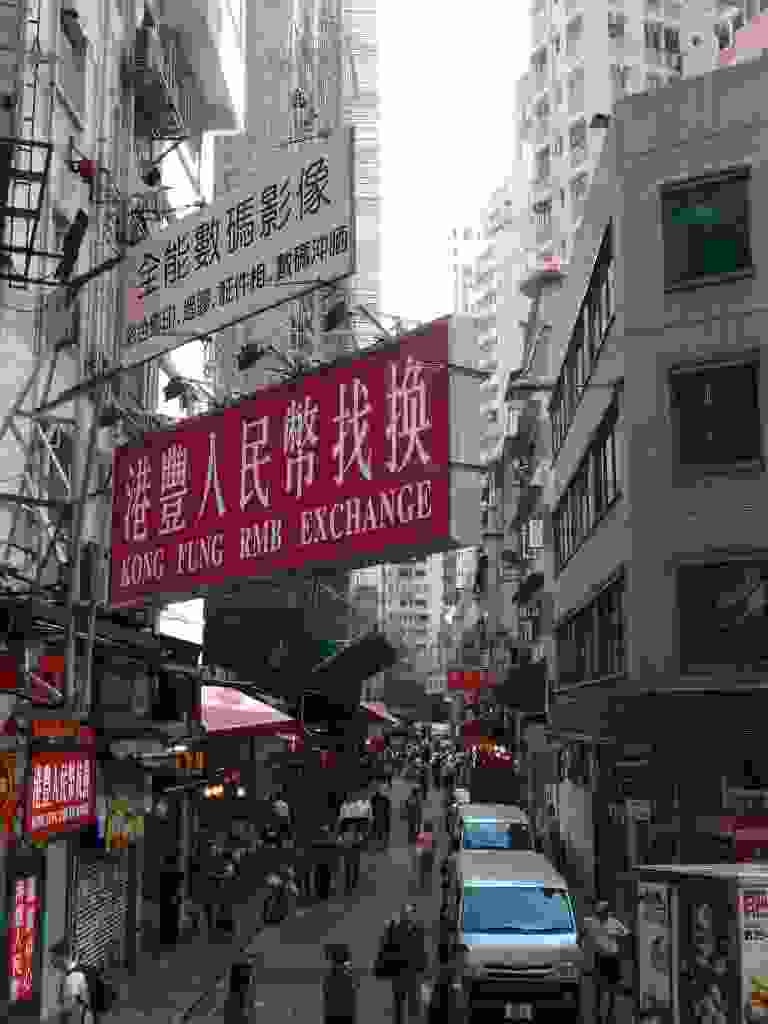
\includegraphics[width=\mywidth]{../wp-content/uploads/2015/10/wpid-oi0000801-e1446026450126-768x1024.jpg} } 
 \newline
 Dernier jour sur Lantau Island pour voir le grand Buddha en bronze \newline
 \newline
\centerline{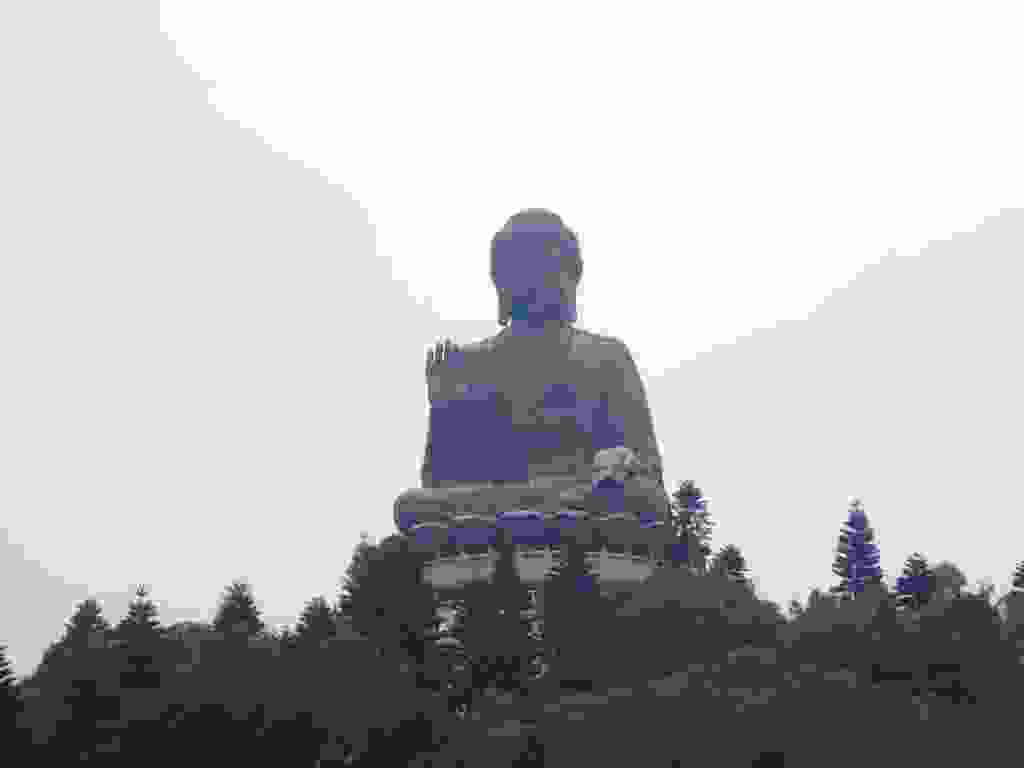
\includegraphics[width=\mywidth]{../wp-content/uploads/2015/10/wpid-oi0001371-1024x768.jpg} } 
 \newline
 \newline
\centerline{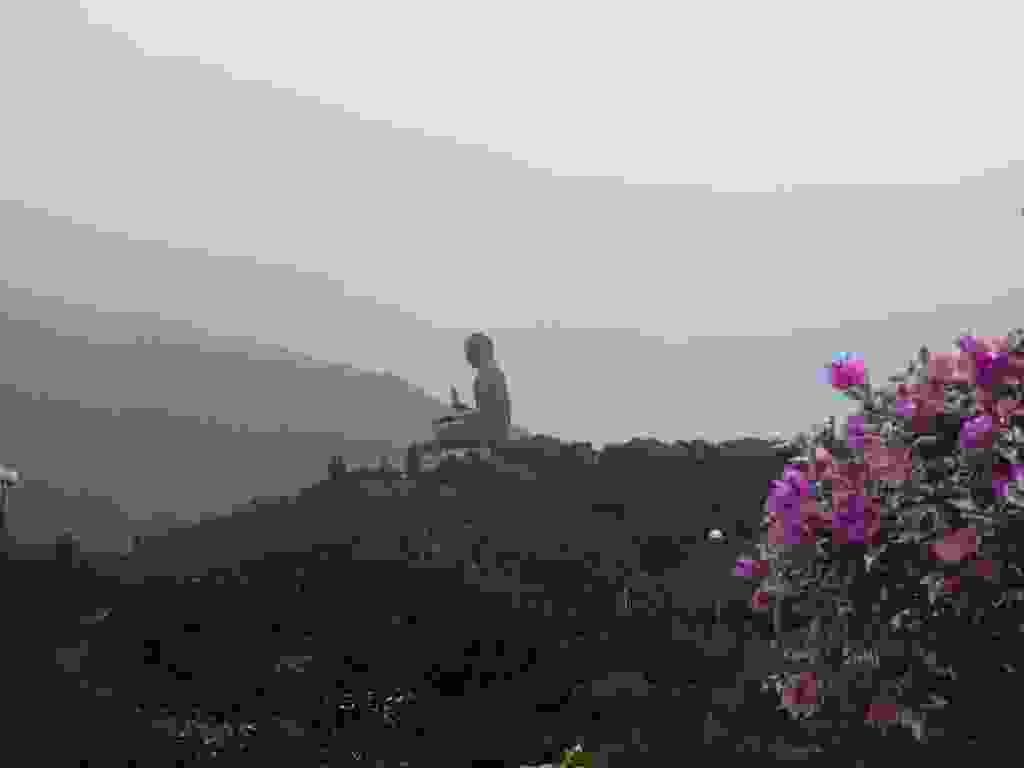
\includegraphics[width=\mywidth]{../wp-content/uploads/2015/10/wpid-oi0001411-1024x768.jpg} } 
 \newline
 \newline
\centerline{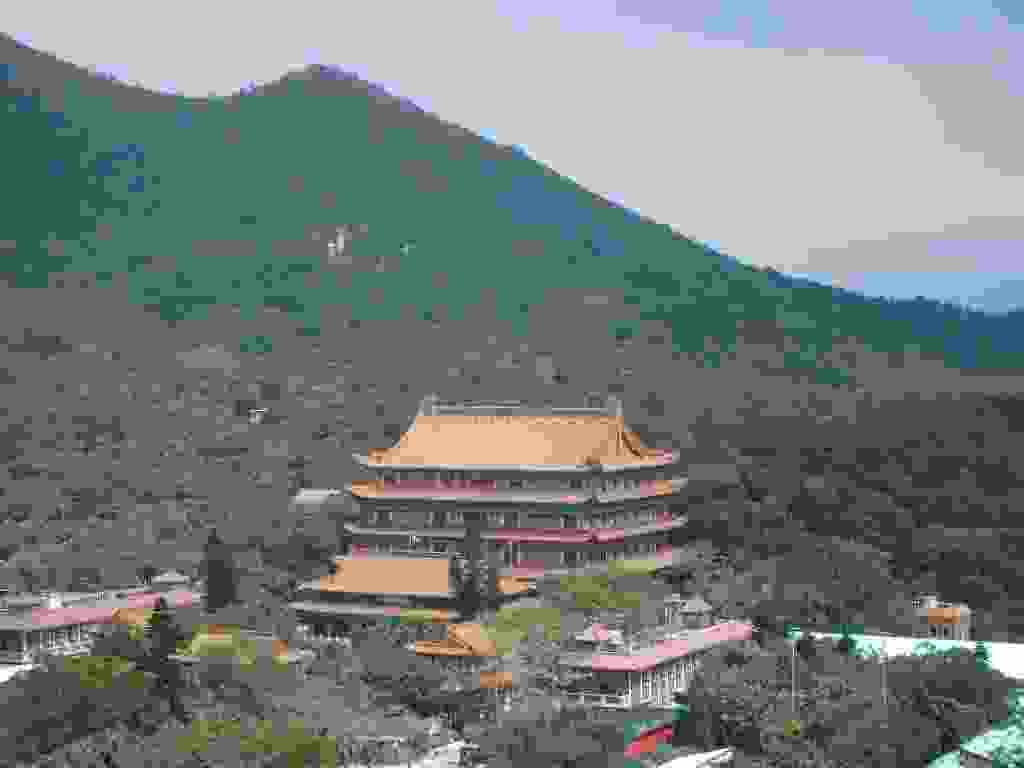
\includegraphics[width=\mywidth]{../wp-content/uploads/2015/10/wpid-oi0001301-1024x768.jpg} } 
 \newline
 Métro pour aller à l'aéroport, destination le sud de Inde \newline
 \newline
\centerline{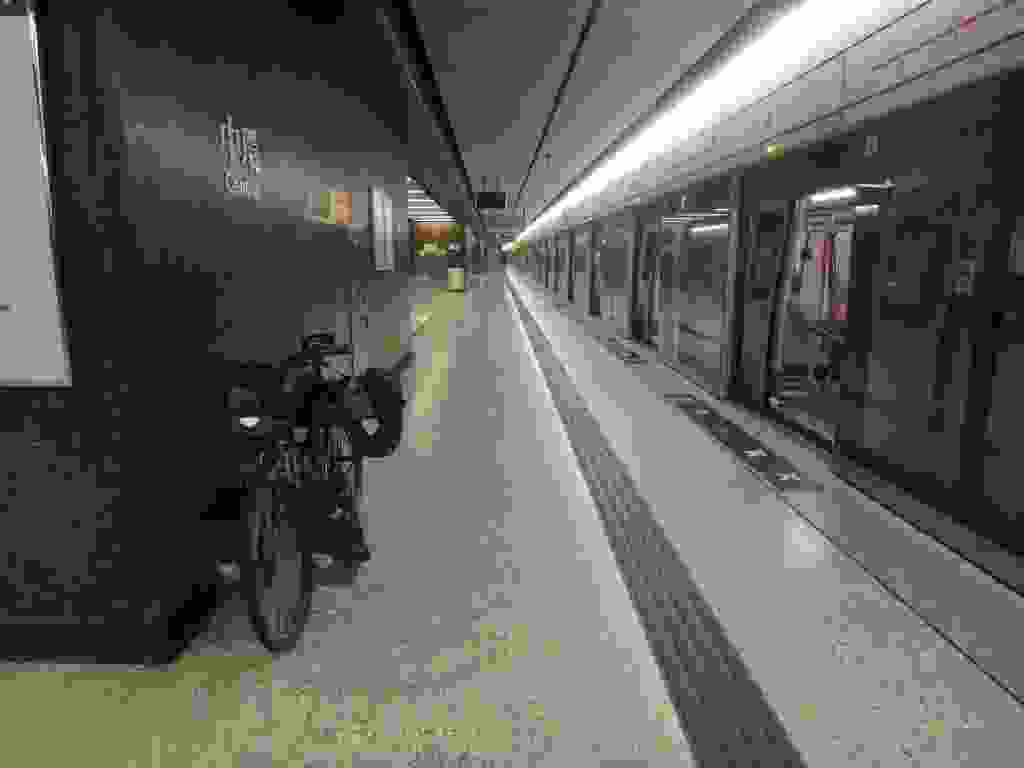
\includegraphics[width=\mywidth]{../wp-content/uploads/2015/10/wpid-oi0001431-1024x768.jpg} } 
 \newline

\newpage
 
